\section{\label{sec:pertth}Matrix elements in perturbation theory}

I illustrate the leading-order, or tree-level, contribution to the smeared nonsinglet matrix element in Fig.~\ref{fig:sqpdf_tree}. In both Figs.~\ref{fig:sqpdf_tree} and \ref{fig:sqpdf1}, I use the following conventions: solid lines represent fermion propagators; double lines are fermion flow kernels; open squares are flow vertices at arbitrary flow time $\tau_1$; gray circles indicate fermion fields at fixed flow time $\tau$; gray squares indicate vertices at fixed flow time $\tau$; and the dashed line is the spatially extended Wilson-line operator.
Note that gauge kernels do not contribute to the smeared nonsinglet quasidistribution at one loop in perturbation theory. The tree-level contribution is given by
\begin{align}
\hm^{(0)} = {} & \frac{1}{2p}\big\langle  \,p,s \,\big| \overline{\chi}(n;\tau)\gamma_\alpha\frac{\lambda^a}{2}\chi(0;\tau) \big|\, p,s \, \big\rangle \nonumber\\
= {} & \frac{1}{2p}e^{ip_zz} e^{-2p^2\tau}\overline{u}^s(p)\frac{\lambda^a}{2}\gamma_\alpha u^s(p),
\end{align}
where I have dropped the arguments of the matrix element for clarity, and I have used
\begin{equation}
\chi(x;\tau) \big | \,p,s \,\big\rangle = e^{-p^2\tau}\psi(x)\big | \,p,s \,\big\rangle =e^{-p^2\tau}e^{ip\cdot x}u^s(p),
\end{equation}
and an analogous relation for the antiquark.

Beyond tree-level, the operator receives radiative corrections that can be written as
\begin{align}
\hm^{(\mathrm{s})}= {} & {\cal Z}_h \hm^{(0)} \nonumber\\
= {} & Z_h^{(1)}(\oz^2,\mu^2\tau) Z_\chi^{(1)}(\mu^2\tau) \big(Z_\psi^{(1)}\big)^{-1}\hm^{(0)}+{\cal O}(\alpha_s^2). \label{eq:matchrel}
\end{align}
Here, $\alpha_s = g^2/(4\pi)$ is the renormalized coupling constant, which is equal to the bare coupling constant to this order and is most naturally evaluated at the scale $\mu^2 = 1/r_\tau^2$. I show the individual one-loop diagrams that contribute to the correction parameter ${\cal Z}_h$ in Fig.~\ref{fig:sqpdf1}. Diagrams (a) to (f) contribute to the operator renormalization parameter, $Z_h$. The wave function renormalization $Z_\psi$ receives contributions from diagram (g). The extra fermion wave function renormalization $Z_\chi$, which receives contributions from diagrams (h), (i) and (j), is automatically removed via the ringed fermions.

The determination of the operator renormalization parameter, $Z_h$, is the central result of this paper. Both the wave function renormalization parameters appear elsewhere (in particular, $Z_\chi$ is calculated in Refs.~\cite{Luscher:2013cpa,Makino:2014taa}); I calculate these contributions for completeness and as a check of my methods and combine these results with $Z_h$ to obtain the complete one-loop correction ${\cal Z}_h$. I show that, in the small flow-time and local vector current limits, the parameter ${\cal Z}_h$ reduces to the corresponding results in the literature \cite{Makino:2014taa,Hieda:2016lly}, a nontrivial check of my results. The existence of a well-defined local vector-current limit for the extended operator is in contrast to, for example, the extended operator in the $\ms$ scheme in the absence of the flow time \cite{Constantinou:2017sej} and is one attractive feature of the smeared quasidistribution.

I split the following discussion into two parts, starting with an analytic study of the UV structure of the matrix elements. This is sufficient to extract $Z_h^{(1)}$ and is possible because I assume the renormalization scale is much larger than the external momentum and set the momentum to zero \cite{Ishikawa:2016znu}. Diagrams (b), (c), (e), and (i) are proportional to the external momentum and therefore vanish in this case. Moreover, the remaining integrals themselves are considerably simplified and become analytically tractable. I regulate the resulting IR divergences with dimensional regularization and demonstrate that these divergences cancel in the matching procedure between the matrix elements in the $\ms$ scheme and at nonzero flow time. In the second part of my discussion, Sec.~\ref{sec:numres}, I numerically evaluate all nine flow-time-dependent diagrams as a function of the external momentum, quark mass, and flow time to illustrate the behavior of the full matrix elements at one loop in perturbation theory.


\subsection{Vertex-type diagrams}

At one loop in perturbation theory, there are three nonvanishing ``vertex-type'' diagrams associated with the extended operator, which are diagrams (a), (d), and (f) in Fig.~\ref{fig:sqpdf1}, and four ``wave-function-type'' diagrams, which are diagrams (g) to (j) in Fig.~\ref{fig:sqpdf1}. At finite Wilson-line length, $z$, the diagrams exhibit the following UV and collinear behavior: diagram (a) is UV finite and logarithmically IR divergent, while diagrams (d) and (f) would be logarithmically UV divergent without the presence of the flow time, which renders them UV finite and IR finite. Thus, I evaluate diagrams (d) and (f) directly in four dimensions, but diagram (a) requires dimensional regularization to regularize the IR behavior of the integral; I choose $d = (4+2\eir)$.  At zero external momentum, the symmetry and dimension of the bare matrix element ensures that the final result is only a function of $\oz^2=z^2/r_\tau^2$ \cite{Radyushkin:2016hsy}, although individual diagrams may also depend on dimensionless combinations of $\mu^2$, $z^2$ and $\tau$. I do not impose any constraints on the functional dependence of any intermediate results, so establishing that the final result depends only on $\oz^2$ is a useful cross-check of the calculation.

To illustrate the calculation, I will consider diagram (a). The calculation of diagrams (d) and (f) proceeds in a very similar manner. At zero external momentum, the contribution to $Z_h$ from this diagram is given by
\begin{equation}
Z^{\mathrm{(a)}} = C_F (-ig_0\gamma_\rho)\! \int_k \frac{e^{-\tau k^2}}{i\kslash}\gamma_\alpha e^{-ik\cdot n} \frac{e^{-\tau k^2}}{i\kslash}(-ig_0\gamma_\sigma)\frac{\delta_{\rho\sigma}}{k^2}.
\end{equation}
Here $C_F = 4/3$ is the color factor; $g_0$ is the bare coupling; all repeated Lorentz indices are summed over; and I define
\begin{equation}
\int_k = \mu^{4-d}\int \frac{\mathrm{d}^dk}{(2\pi)^d}.
\end{equation}

The Lorentz structure of the numerator is straightforward and, using the Schwinger representation for the denominator, this integral becomes
\begin{align}\label{eq:hma}
Z_h^{\mathrm{(a)}} = {} &  g_0^2C_F \frac{\mu^{4-d}}{(2\pi)^d} \int_0^\infty\mathrm{d}\alpha\,\frac{\alpha}{2} \nonumber \\
& \times \int \mathrm{d}^dk\, N_\alpha(k,d)e^{-(2\tau+\alpha) k^2} e^{-ik\cdot n}.
\end{align}
The numerator $N(k,d)$ depends, at finite flow time and spatial separation, on the choice of Lorentz structure in the original matrix element. Introducing momentum components parallel and perpendicular to the spacelike separation, $k_z$ and $k_\perp=(k_x,k_y,k_t)$, respectively, this numerator is given by
\begin{equation}
N(k,d) \equiv (2-d)(k_z^2-k_\perp^2)
\end{equation}
for the choice $\gamma_\alpha = \gamma_z$ in $\hm^{(s)}$ in Eq.~\eqref{eq:hdef} and
\begin{equation}
N(k,d) \equiv (2-d)\left(\displaystyle\frac{3-d}{d-1}k_\perp^2 - k_z^2\right)
\end{equation}
otherwise.

The momentum integral in Eq.~\eqref{eq:hma} can be carried out by integrating over $k_z$ and $k_\perp$ individually, leaving a Schwinger parameter integral over $\alpha$ that can be done analytically, giving
\begin{align}
Z_h^{\mathrm{(a)}} = {} & \left(\frac{g_0}{4\pi}\right)^2C_F\bigg[\frac{1}{\eir} -\gE-\log\left(\pi \mu^2z^2\right) +3\nonumber\\
{} - \frac{3}{\oz^4} & \Big(e^{-\oz^2}-1\Big)- \frac{1}{\oz^2} \left(4-e^{-\oz^2}\right)+\ei{-\oz^2}\bigg], \label{eq:hta1}
\end{align}
and
\begin{align}
Z_h^{\mathrm{(a)}} = {} &\left(\frac{g_0}{4\pi}\right)^2C_F \bigg[\frac{1}{\eir}-\gE-\log\left(\pi \mu^2z^2\right)+1\nonumber\\
&{} -\frac{1}{\oz^4}\Big(1-e^{-\oz^2}(1+\oz^2)\Big)+\ei{-\oz^2} \bigg], \label{eq:hta2}
\end{align}
respectively. Here, $\ei{z}$ is the exponential integral
\begin{equation}
\ei{z} = -\int_{-z}^\infty \frac{e^{-t}}{t}\mathrm{d}t.
\end{equation}
As one would expect, the gradient flow does not affect the IR structure of this diagram (see the Appendix for the equivalent result without the presence of the gradient flow).

I treat the other diagrams, (d) and (f), in a similar fashion and find
\begin{align}
Z_h^\mathrm{(d)} = {} & 2 g_0^2C_F\frac{\pi^2}{(2\pi)^4}\int_0^\infty\mathrm{d}\alpha\,\frac{\alpha}{(\alpha+2\tau)^2}\nonumber \\
{} & \qquad \qquad\qquad\times \left(1-e^{-z^2/(4(\alpha+2\tau))}\right),\\
Z_h^\mathrm{(f)} = {} & g_0^2C_F \frac{\pi^{d/2}}{(2\pi)^4}\int_0^\infty\mathrm{d}\alpha\,\frac{1}{(\alpha+2\tau)^{3/2}} \nonumber \\
\times {} & \int_0^\infty\mathrm{d}\beta\frac{1}{\sqrt{\alpha+\beta+2\tau}}\left(e^{-z^2/(4(\alpha+\beta+2\tau))}-1\right).
\end{align}
The results are
\begin{align}
\!\!Z_h^\mathrm{(d)} = {} & -\left(\frac{g_0}{4\pi}\right)^2C_F \cdot2\bigg[1-\gE-\log\left(\oz^2\right)+\ei{-\oz^2} \nonumber \\
{} & \qquad  + \frac{1}{\oz^2}\left(e^{-\oz^2}-1\right)\bigg], \label{eq:htd}\\
\!\!
Z_h^\mathrm{(f)} = {} & \left(\frac{g_0}{4\pi}\right)^2C_F \cdot2\bigg[\gE+\log\left(\oz^2\right)- \ei{-\oz^2}  \nonumber \\
{} & \quad {-} 2\left(e^{-\oz^2}-1\right) -2\sqrt{\pi\oz^2}\erf{\sqrt{\oz^2}}\bigg],
\label{eq:htf}
\end{align}
where $\erf{z}$ is the error function
\begin{equation}
%\Gamma(a,z) = {} & \int_z^\infty t^{a-1}e^{-t}\mathrm{d}t,\\
\erf{z} = \frac{2}{\sqrt{\pi}}\int_0^z e^{-t^2}\mathrm{d}t.
\end{equation}
This term is the one-loop contribution to the expected power divergence and scales linearly with the length of the Wilson line for $\oz \gg 1$.

\subsection{Wave-function-type diagrams}

The ``wave-function-type'' diagrams are diagrams (g), (h), and (j) in Fig.~\ref{fig:sqpdf1} [diagram (i) is proportional to the external momentum]. The contribution from diagram (g) is just the standard quark wave function renormalization, which will cancel exactly in the one-loop matching relation between the smeared and $\ms$ distributions, because it is independent of the flow time.
In general, this diagram vanishes in dimensional regularization for vanishing external momentum and in the absence of any other scales, but it is helpful to expose the UV and IR divergences by introducing a separation scale, and I discuss this in more detail in the Appendix.

The divergent pieces of the flow-time-dependent diagrams (h) and (j) are removed through the use of ringed fermions, which incorporates the extra fermion renormalization $Z_\chi$ associated with the fermions at finite flow time. Diagrams (h) and (j) include flow vertices that occur at arbitrary flow times $\tau_i$ and must be integrated from zero to $\tau$. The contributions from these diagrams are represented by
\begin{align}
Z_h^\mathrm{(h)} = {} & 2 g_0^2C_F\cdot 2\int_0^\tau \mathrm{d}\tau_1
\int_k \frac{e^{-2k^2\tau_1}}{k^2} \nonumber \\
= {} & \left(\frac{g_0}{4\pi}\right)^2  C_F \cdot 2\left[\frac{1}{\euv}
+1+\log\big(8\pi\mu^2\tau\big)\right], \label{eq:hth}\\
Z_h^\mathrm{(j)}{} & (\mu^2\tau) = {-} 2g_0^2C_F  d\int_0^\tau \mathrm{d}\tau_1\int_k\frac{e^{-2k^2\tau_1}}{k^2} \nonumber \\
= {} & -\left(\frac{g_0}{4\pi}\right)^2C_F \cdot 4\left[\frac{1}{\euv} +\frac{1}{2} + \log(8\pi\mu^2\tau)\right]\label{eq:htj},
\end{align}
where I have included a factor of 2 to account for the corresponding antiquark corrections. These contributions, which are independent of the nonlocal operator structure and are canceled by terms in $Z_\chi$, were first calculated for local quark bilinear operators in Ref.~\cite{Endo:2015iea}.

\subsection{One-loop renormalization parameter}

Drawing together these results, I obtain the one-loop expression for the parameter $Z_h$,
\begin{equation}
Z_h^{(1)} =   1 + \frac{\alpha_s}{3\pi}\Big[Z_h^\mathrm{(a)}+Z_h^\mathrm{(d)} +Z_h^\mathrm{(f)}+Z_h^\mathrm{(g)}+Z_h^\mathrm{(h)}+Z_h^\mathrm{(j)}\Big],
\end{equation}
which is
\begin{align}
Z_h^{(1)} = & {} 1 + \frac{\alpha_s}{3\pi}\bigg[-\frac{3}{\euv}+3\gE+3\log\left(\oz^2\right) -3\operatorname{Ei}(-\oz^2)\nonumber\\
{}  -4&\sqrt{\pi\oz^2}\erf{\sqrt{\oz^2}} -3\log(8\pi\mu^2\tau)+a(\oz^2)\bigg],
\end{align}
where
\begin{equation}
a(\oz^2) =  5 + \frac{3}{\oz^4} \Big(1-e^{-\oz^2}\Big)- \frac{1}{\oz^2} \left(2+e^{-\oz^2}\right)-4e^{-\oz^2},
\end{equation}
for $\gamma_\alpha = \gamma_z$ and
\begin{equation}
a(\oz^2) =  3 - \frac{1}{\oz^4} \Big(1-e^{-\oz^2}\Big)+ \frac{1}{\oz^2} \left(2-e^{-\oz^2}\right)-4e^{-\oz^2}
\end{equation}
otherwise. These expressions are the central results of this work.

\subsubsection{Asymptotic behavior}
These one-loop expressions satisfy a number of cross-checks, based on the structure expected in the asymptotic regimes $\oz \ll1 $ and $\oz \gg 1$, which correspond to the local vector-current and small flow-time limits, respectively.

\paragraph{Vector-current limit} In principle, in contrast to the dimensionally regularized case (see the Appendix), there are no contact terms in the limit of vanishing quark-field separation $z\to 0$ \cite{Constantinou:2017sej}, provided one has regulated the IR divergences through an appropriate regulator, such as an IR cutoff or external momentum. In this case, one could directly take the limit $\oz\to 0$. Here, however, I have used dimensional regularization for the IR divergences, which now manifest in a logarithmic dependence on $\mu^2z^2$, and this complicates the procedure. It is simplest to examine the $\oz\ll 1$ regime at the level of each integrand, in which case one finds $Z_h^\mathrm{(d)}=Z_h^\mathrm{(f)}=0$ and
\begin{equation}
\lim_{\oz \to 0}Z_h^\mathrm{(a)} =  \left(\frac{g_0}{4\pi}\right)^2C_F \left[\frac{1}{\eir}+\frac{1}{2} - \log\left(8\pi\mu^2\tau\right)\right],
\end{equation}
independent of the choice of the matrix $\gamma_\alpha$ in the original matrix element, as expected.

Combining this result with the expressions for diagrams (h) and (j), which are independent of the spatial separation $z$ (but not, of course, the flow time $\tau$), I find
\begin{equation}
\lim_{\oz \to 0}Z_h^{(1)} = \left(\frac{g_0}{4\pi}\right)^2C_F \left\{\frac{1}{2}+\frac{1}{\eir}-\frac{3}{\euv} + \log\left(8\pi\mu^2\tau\right)\right\},\label{eq:hoztozero}
\end{equation}
As I show in the next section, when combined with $Z_\psi$ and $Z_\chi$, the parameter $Z_h^{(1)}$ reduces to the local vector-current result of Ref.~\cite{Hieda:2016lly}, an important check of the calculation.

\paragraph{Small flow-time limit} In the small flow-time limit, one anticipates that the diagrams reduce to the expressions obtained in the $\ms$ scheme. Diagram (a) reduces to
\begin{equation}
Z_h^{(a)}  \stackrel{\oz \gg 1}{\simeq}\left(\frac{g_0}{4\pi}\right)^2C_F \bigg[\frac{1}{\eir} + C^{(\infty)}_\alpha-\gE-\log(\pi\mu^2z^2) \bigg],
\end{equation}
where $C^{(\infty)}_z = 3$ and $C^{(\infty)}_\perp = 1$. These results are in exact agreement with the $\ms$-scheme expressions in Eq.~\ref{eq:ha_dr}.
Taking $\oz \gg 1$, diagrams (d) and (f) become
\begin{align}
Z_h^\mathrm{(d)}\!\! \stackrel{\oz \gg 1}{\simeq} {} & \!\!\!{-}\left(\frac{g_0}{4\pi}\right)^2C_F 2\bigg[1-\gE-\log(\oz^2) \bigg],\\
Z_h^\mathrm{(f)}\!\! \stackrel{\oz \gg 1}{\simeq} {} & \!\!\!\left(\frac{g_0}{4\pi}\right)^2C_F 2\bigg[1+\gE+\log(\oz^2)  +\left(1-2\sqrt{\pi}\oz\right) \bigg].
\end{align}
The contribution to diagram (f) in parentheses is the linear divergence that must be subtracted before comparison can be made to the calculation carried out with dimensional regularization. Removing this contribution, the sum of these two diagrams is
\begin{equation}
\left(Z_h^\mathrm{(d)} +Z_h^\mathrm{(f)}\right)\stackrel{\oz \gg 1}{=} 4\left(\frac{g_0}{4\pi}\right)^2C_F,\label{eq:hoztoinfty}
\end{equation}
in agreement with the sum of Eqs.~\eqref{eq:hd_dr} and \eqref{eq:hf_dr}. In short, the small flow-time limit of $Z_h$ exactly matches the corresponding result directly calculated in the $\ms$ scheme, as one would expect.


\subsection{One-loop smeared matrix element}

We can now write down the complete smeared matrix element, $\hm^{(\mathrm{s})}$ at one loop in perturbation theory, by combining the wave function renormalization $Z_\psi$ and $Z_\chi$ \cite{Luscher:2013cpa,Makino:2014taa} with the results for $Z_h$ from the previous section. Recalling Eq.~\eqref{eq:matchrel}, the one-loop matrix element is
$\hm^{(\mathrm{s})} = {\cal Z}_hh^{(0)}$, where
\begin{align}
{\cal Z}_h^{(1)} = & {} 1 + \frac{\alpha_s}{3\pi}\bigg[3\log\left(\oz^2\right) +6\gE-3\log(4\pi)-\log(432)\nonumber \\
{} &  -3\operatorname{Ei}(-\oz^2) -4\sqrt{\pi\oz^2}\erf{\sqrt{\oz^2}}+a(\oz^2)\bigg]
\end{align}
and here
\begin{align}
c(\oz^2) = {} & 3\left[3+\frac{1}{\oz^2}\left(e^{-\oz^2}-2\right)+\frac{1}{\oz^4}\left(1-e^{-\oz^2}\right)\right] ,  \label{eq:cmuz}\\
c(\oz^2) = {} & 7 +\frac{1}{\oz^2}\left(3e^{-\oz^2}-2\right) +\frac{1}{\oz^4}\left(e^{-\oz^2}- 1\right),\label{eq:cmuperp}
\end{align}
for $\gamma_\alpha = \gamma_z$ and $\gamma_\alpha = \gamma_\perp$, respectively. I note that the IR divergences in the vertex correction of diagram (a) and the wave function renormalization, diagram (g), have canceled. This matches the IR behavior in the $\ms$ scheme, Eq.~\eqref{eq:zhmsbar}, and demonstrates that the gradient flow does not modify the IR behavior of the quasidistribution. Moreover, the total one-loop result is UV finite (that is, there are no poles in $\euv$), as is guaranteed for nonzero flow time, provided one uses ringed fermions. The logarithmic terms combine in such a way that all dependence on $\mu$ has been eliminated, leaving only $\log(\oz)$. There is a linear divergence generated by the Wilson-line self-energy, diagram (f), that scales as $z/\sqrt{\tau}$, as one would expect on dimensional grounds. At higher orders in perturbation theory, one anticipates that this divergence exponentiates in the form $e^{-cz/\sqrt{\tau}}$.

I plot both ${\cal Z}_{\mathrm{sub}}^{(z)}(\oz^2)$ and ${\cal Z}_{\mathrm{sub}}^{(\perp)}(\oz^2) $ as functions of $\oz$ in Fig.~\ref{fig:Zozplot}, represented by the purple and blue curves, respectively. I have removed the linear divergence, which would otherwise dominate for values of $\oz\simeq 2$, as illustrated by the dot-dashed gray line, which shows ${\cal Z}^{(z)}(\oz^2)$ including the linear divergence, denoted by ${\cal Z}^{(z)}(\oz^2)$ in the legend. I also plot the asymptotic behavior in the $\oz \ll 1$ and $\oz \gg 1$ regimes as orange dashed lines.
\begin{figure}
\centering
\caption{Renormalization parameter ${\cal Z}_h^{\mathrm{sub}}$ for $\gamma_\alpha=\gamma_z$ and $\gamma_\alpha = \gamma_\perp$ as a function of $\oz$, where the superscript ``$\mathrm{sub}$'' indicates that the linear divergence has been subtracted. The dot-dashed gray line is ${\cal Z}_h$ including the linear divergence in $\oz$, denoted by ${\cal Z}_h^{\mathrm{div}}$ in the legend. I plot the asymptotic behavior for $\oz \ll 1$ and $\oz \gg 1$, from Eqs.~\eqref{eq:veclimit} and \eqref{eq:zsmalltau} as orange dashed lines.}
\label{fig:Zozplot}
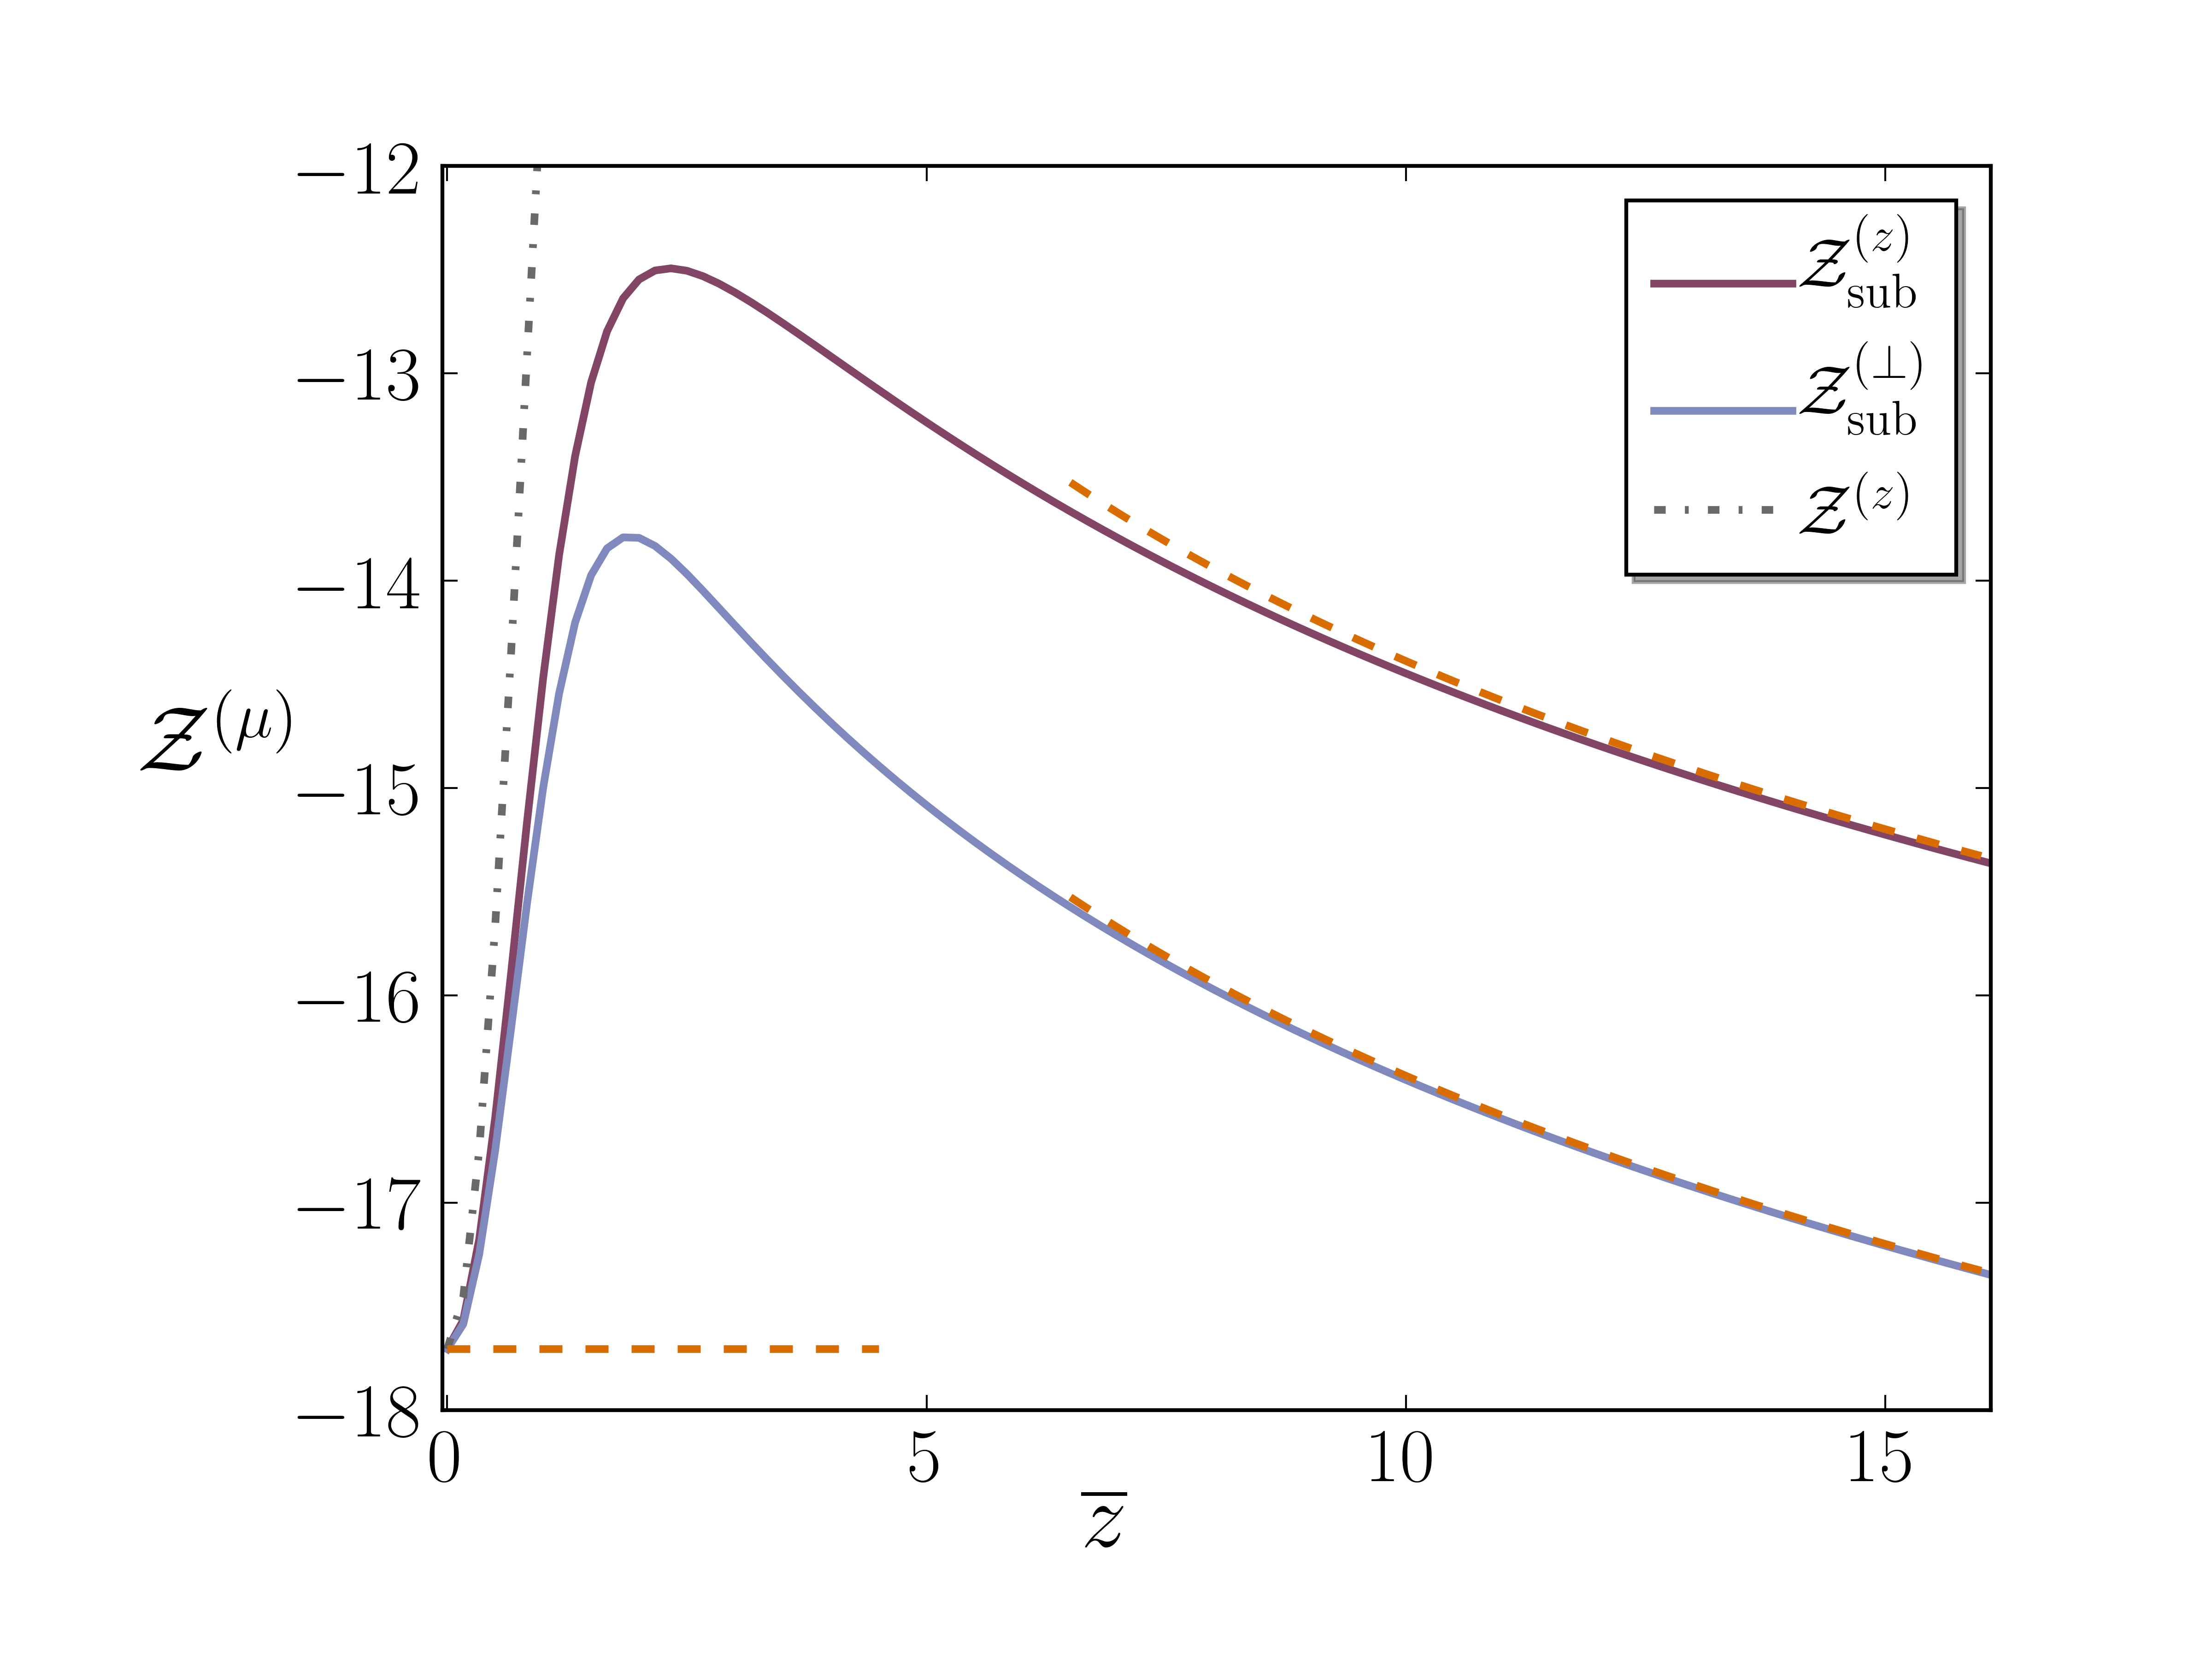
\includegraphics[width=0.47\textwidth,keepaspectratio]{images/zmu.png}
\end{figure}

\paragraph{Vector-current limit} In contrast to the matrix element in dimensional regularization, the limit of vanishing spatial separation of the quark fields, $\oz\to 0$, is well defined and is given by
\begin{equation}\label{eq:veclimit}
\lim_{\oz\to0}{\cal Z}_h  = \frac{1}{2}-\log(432),
\end{equation}
independent of the choice one makes for $\gamma_\alpha$ and in exact agreement with the vector-current result of \cite{Hieda:2016lly}. This result exhibits a feature characteristic of composite operators constructed from ringed fermions: perturbative corrections are finite, as they must be for a conserved vector current, but not necessarily zero (compare, for example, with the nonsinglet axial-vector current defined in Ref.~\cite{Endo:2015iea}).


\paragraph{Small flow-time limit} Conversely, the small flow-time expansion gives
\begin{equation}\label{eq:zsmalltau}
{\cal Z}_h^{\mathrm{(sub)}} \stackrel{\oz\gg1}{\simeq} b - \gE - \log(432) - \log(\oz^2),
\end{equation}
with $b = 9$ and $b=7$, for $\gamma_\alpha = \gamma_z$ and $\gamma_\alpha = \gamma_\perp$, respectively. In this regime, the parameter ${\cal Z}_h^{\mathrm{sub}}(\oz^2)$ depends only logarithmically on $\oz$, and therefore satisfies a relation akin to the usual renormalization-group equation \cite{Monahan:2015lha}:
\begin{equation}\label{eq:zsubRG}
\left[\frac{\mathrm{d}}{\mathrm{d}\log\oz^2} +\gamma_{\oz}\right]{\cal Z}_h^{\mathrm{sub}}(\oz^2) = 0.
\end{equation}
Here, $\gamma_{\oz} = \gamma_{\oz}^{(1)}\alpha_s+{\cal O}(\alpha_s^2)$, with $\gamma_{\oz}^{(1)}=1$, is analogous to the usual anomalous dimension. Beyond one loop in perturbation theory, a complete renormalization-group analysis would necessarily take into account the implicit scale dependence of the coupling constant $\alpha_s(\mu)$. A renormalization-group trajectory is then a path in the two-dimensional space $(\oz,\mu)$, which can be simplified by tying the two scales together by choosing, for example, $\mu = 1/r_\tau$ \cite{Monahan:2015lha}. In principle, this could provide an opportunity to construct a nonperturbative step-scaling method for the matrix element $\hm^{(\mathrm{s})}(\oz^2)$, which would connect lattice calculations at hadronic scales to a high scale at which the matching to the $\ms$ scheme can be carried out without significant perturbative truncation uncertainties. Equation \eqref{eq:zsubRG} only holds in the small flow-time regime, however, which, from Fig.~\ref{fig:Zozplot}, applies for $\oz \simeq 10$, at least at one loop in perturbation theory. Imposing this constraint throughout the entire step-scaling procedure may not be feasible for current lattices, but systematic uncertainties associated with deviations from the small flow-time expectation can be studied nonperturbatively.


\subsection{Matching in coordinate space}

With the complete one-loop expression for the smeared quasidistribution in hand, I can match the results to the renormalized matrix element in the $\ms$ scheme, $\hm^{\ms}(\mu^2z^2)$ (see the Appendix). Writing
\begin{equation}
\hm^{\ms}(\mu^2z^2) = {\cal C}_h^{\mathrm{sub}}(\mu^2z^2,\oz^2)\hm^{(\mathrm{s})}(\oz^2),
\end{equation}
the matching factor is given by
\begin{align}
%\!\!{\cal C}_h^{\mathrm{sub}}(\mu^2z^2,\oz^2){} &  = 1 +\frac{\alpha_s}{3\pi}\Big[3\overline{c}-c(\oz^2)+7\gE \nonumber\\
%\! +3\log(432) -{} & \ei{-\oz^2} +\log\left(\oz^2\right)+3\log\left(\mu^2z^2\right) \Big].\\
\!\!{\cal C}_h^{\mathrm{sub}}(\mu^2z^2,\oz^2){} &  = 1 +\frac{\alpha_s}{3\pi}\Big[a(\oz^2)-3\overline{c} -\log(432)\nonumber\\
 - 3\ei{-\oz^2} {} & -3\log\left(8\pi\mu^2t\right) -4\sqrt{\pi\oz^2}\erf{\sqrt{\oz^2}}\Big].
\end{align}
Here $c(\oz^2)$ is given in Eqs.~\eqref{eq:cmuz} and \eqref{eq:cmuperp}, $\overline{c} =5/3$, and $\overline{c} =7/3$. In general, the linear divergence will be subtracted nonperturbatively and I have removed this contribution from the matching relation, indicated by the subscript ``$\mathrm{sub}$.''
At zero external momentum, this matching parameter is real; at finite external momentum, discussed in the next section, the matching parameter becomes imaginary  \cite{Constantinou:2017sej}.
